\chapter{SYSTEM DESIGN}
\hspace{0.5cm}
The design of the AI-Powered Code Documentation Generator is elaborated on in this chapter, emphasizing the organization and structure of system components and the travel of the source code through the pipeline process stages of language identification, feature extraction, AST analysis and the LLM engine until accurate and structured documentation is eventually generated. A modular design approach is used, where every component has an individual purpose in the entire system. This chapter also discusses how the modules interact with each other and how the data flow from the input (source code) to the output (documentation). 
\section{System Architecture}
\hspace{0.5cm}
As depicted in Figure 5.1, the architecture of the proposed system represents an AI-driven pipeline for automated code documentation. The process begins when the user provides source code, either by uploading a file or supplying a repository URL. Initially, the input is analyzed by the Language Detection Module to determine the programming language, ensuring that subsequent parsing is accurate. Following this, the system conducts two parallel processes: the Text Feature Extraction Module captures surface-level code features, while the AST Analysis Module generates a structured representation of the code’s components.

\par The AST output is then sent to the Graph Building Module, where a graph is constructed with nodes representing functions or classes and edges representing relationships such as function calls and dependencies. The outputs from the Text Analysis Module, AST Module and Graph Building Module are then combined in the Feature Fusion Module to produce a comprehensive representation that integrates the textual, structural and relational aspects of the code.
\par This integrated representation is then fed into the LLM Module, which produces human-readable documentation. The Documentation Module organizes this content into various document formats and delivers the finalized documentation to the user.
\newline


\FloatBarrier
\begin{figure}[htbp]
    \centering
    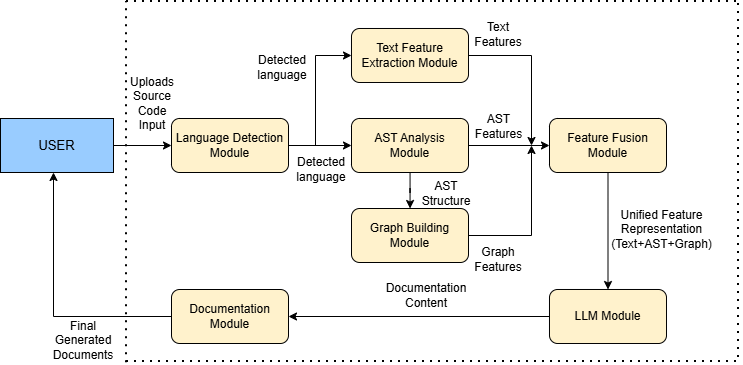
\includegraphics[width=\textwidth]{tex/Untitled Diagram-Page-2.drawio (3).png}
    \caption{Architecture Diagram of the AI-Powered Code Documentation Generator.}
    \label{fig:architecture}
\end{figure}
\FloatBarrier



\section{Data Flow Diagram (DFD)}
\hspace{0.5cm}Figures 5.2 and 5.3 illustrate the data flow diagrams of the proposed system, showing the complete movement of data throughout the automated code documentation generation process.
\subsection{DFD Level 0}

\hspace{0.5cm}Figure 5.2 demonstrates the Level 0 Data Flow Diagram (DFD) of the AI-Powered Code Documentation Generator. The user provides source code to the system, which uses AST analysis to extract essential details such as functions, classes, imports and other relationships. Based on this extracted information, the AI generates structured documentation and delivers it to the user.
\hspace{0.3cm}
\FloatBarrier
\begin{figure}[h]
	\centering
	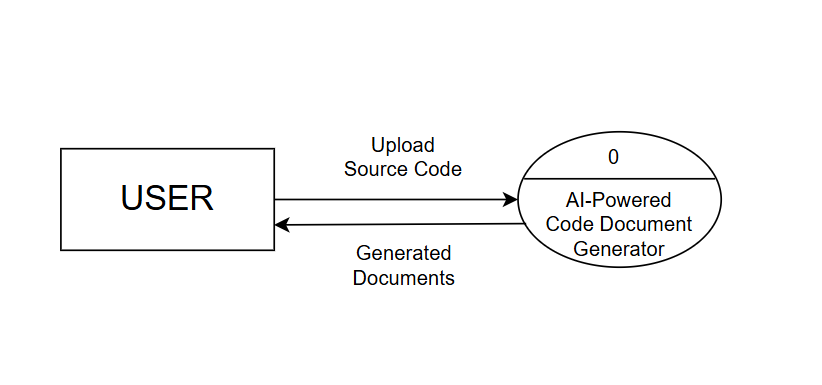
\includegraphics[scale=0.6]{tex/Screenshot 2026-04-13 101331.png}
	\caption{Data Flow Diagram Level 0.}
	\label{lvmh2}
\end{figure}
\subsection{DFD Level 1}


\hspace{0.5cm}Figure 5.3 presents the internal processing of the AI-Powered Code Document Generator as a Level 1 DFD. The process begins when the user uploads the source code and the Language Detection Module identifies the programming language based on the file extension. Once the language is detected, two parallel streams occur: the Text Feature Extraction Module extracts textual information and code metrics, generating text data, while the AST Extraction Module parses the code to create its abstract syntax tree, representing its structural organization. The AST is then passed to the Graph Feature Extraction Module to produce graph-based features capturing relationships among functions, classes and method calls. All features are merged in the Feature Fusion Module, which is subsequently processed by the LLM Engine (Ollama) to generate a natural language description of the source code. Finally, the Document Generation Module formats this output into structured documentation for the user.

\hspace{0.3cm}
\FloatBarrier
\begin{figure}[htbp]
    \centering
    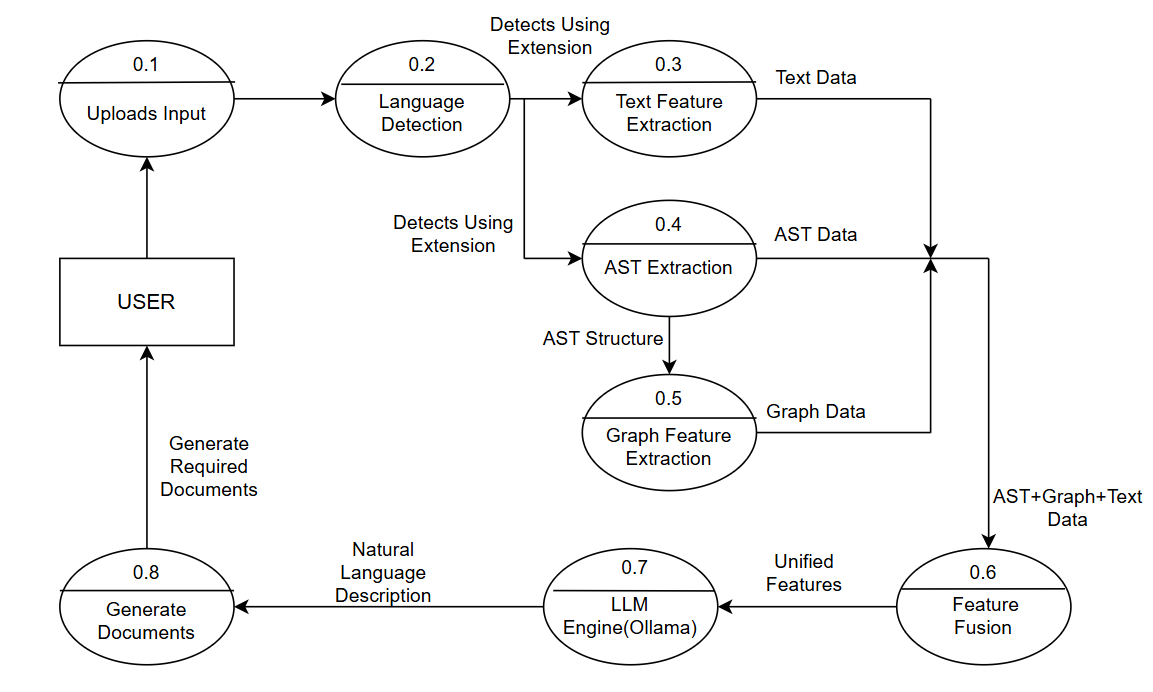
\includegraphics[width=\textwidth,keepaspectratio]{tex/Screenshot 2026-03-11 142330.png}
    \caption{Data Flow Diagram Level 1.}
    \label{fig:dfd1}
\end{figure}

\newpage


\section{List of Modules}
\hspace{0.5cm}
The AI-Powered Code Documentation Generator is composed of the following modules:
\begin{itemize}
    \item User Interface Module
    \item Language Detection Module
    \item Text Feature Extraction Module
    \item AST Analysis Module
    \item Graph Building Module
    \item Feature Fusion Module
  
    \item LLM Engine Module
    \item Documentation Output Module
\end{itemize}

\subsection{User Interface Module}
\hspace{0.5cm}
This module serves as the main interface between the user and the system. It allows users to provide source code files, project directories or repository URLs and access both the generated documentation and the results of intermediate analysis. The interface ensures smooth navigation through each step of the process, making the analysis workflow seamless for the user.

\subsection{Language Detection Module}
\hspace{0.5cm}
The Language Detection Module identifies the programming language of the uploaded source code by analyzing file extensions and syntax. This detected language guides the system in selecting the appropriate parsing strategies and analysis methods. Accurate identification ensures correct AST generation and feature extraction, allowing the system to efficiently process multi-language projects and improving overall flexibility and adaptability.

\subsection{Text Feature Extraction Module}
\hspace{0.5cm}
This module extracts text-based features from the source code, calculating metrics such as the number of lines, tokens, comments, identifiers and keywords. It also identifies import statements, revealing external libraries and dependencies used in the project. These features are critical for generating project-level documentation, including README files and technology stack summaries, providing a comprehensive overview of the codebase. The module operates independently of language-specific syntax, making it fast and lightweight.

\subsection{AST Analysis Module}
\hspace{0.5cm}
This module analyzes the structure of the source code using an AST. It provides detailed insights into the internal structure of the code by extracting classes, functions, parameters, return types, variables, imports and function calls. As a core module, it ensures accurate and meaningful documentation based on the code itself rather than assumptions. It also supports language-aware analysis to enhance extraction accuracy and efficiency.

\subsection{Graph Building Module}
\hspace{0.5cm}
This module constructs a semantic graph from the AST. Nodes represent code elements such as files, classes and functions, while edges indicate relationships like function calls, imports and inheritance. The graph provides a clear visualization of interactions among code components, illustrating data flow and module dependencies. It also supports deeper analysis, including the identification of recursion, unused functions and critical components.

\subsection{Feature Fusion Module}
\hspace{0.5cm}
This module integrates textual features, AST-based structural features and graph-based relational features. Textual features provide specific information, AST features detail the functionality of each component and graph features illustrate the relationships between components. By combining all these features, the system can generate more accurate and comprehensive documentation, ensuring that no information is lost during processing.

\subsection{LLM Engine Module}
\hspace{0.5cm}
This module uses a LLM to create human-readable documentation. The input to the module consists of feature summaries created from the AST, text and graph analysis. The model uses the structural and contextual information to create accurate documentation about the functionality of the code and the architecture of the system. This ensures the readability, accuracy and appropriateness of the created documentation. The level of detail in the documentation depends on the complexity of the input code.

\subsection{Documentation Output Module}
\hspace{0.5cm}
This module handles structuring the generated documentation in an organized layout, covering areas such as project overview, architecture, API documentation and module-level details. It ensures consistency in presentation, enhancing readability and usability. The documentation can be exported to formats like Markdown, making integration with existing development workflows easier and supporting efficient sharing and management.
\newline
\par In this chapter, the overall system design of the AI-Powered Code Documentation Generator is discussed, including the system architecture, the functionality of its various modules and the complete data flow. This design enables each module to process the source code independently while ensuring that the analysis and documentation generation proceed systematically and cohesively. With the system’s design and architecture established, the next chapter will cover the implementation aspects, detailing the development of each module and how they integrate to achieve the intended functionality.
